% -*- mode:LaTex; mode:visual-line; mode:flyspell; fill-column:75-*-

\chapter{Background \& Related Work} \label{chapBackground}
\section{Motivation}
Forests impact many aspects of our life on earth, ranging from the composition of the atmosphere, purification of water, moderating local temperature, and contributing to fire risk \cite{IPCC2019ClimateReport}. Unfortunately, they are under threat from a variety of factors including climate change, invasive species, fire, and direct human pressures. This is causing forests to change at an unprecedented rate. In light of these rapid changes, it is critical that we have up-to-date information to inform decisions such as habitat preservation, sustainable timber operations, forest fire mitigation, and carbon sequestration. In this work we specifically study aspects of forest fire mitation and carbon sequestration, though the approaches aim to be generic enough to scale to other applications. 

\subsection{Forest Fire Mitigation} 
Destructive forest fires have increased dramatically over the past decades \cite{spreading_like_wildfire, ayanz2021, nfn2022}. This is due in large part to climate change, which leads to hotter and drier weather along with stronger winds \cite{spreading_like_wildfire}. This has also led to increased forest mortality from pests expanding their range, such as the mountain pine beetle in the Western US \cite{Jenkins2014AndFuels}. Humans have also contributed more directly to fires by suppressing small fires which causes fuel to build up over time. Finally, there is an increase in ignition sources from careless human activity and infrastructure such as power lines. These fires are now more dangerous to humans and property because of their scale and speed as well as increasing habitation in close proximity to forests, termed the urban-woodland interface. The ecological consequences of fire are also increasingly dire. Historical fires were a natural part of the ecosystem and the vegetation was able to regenerate due to surviving trees and un-burned seeds. The intensity of modern fires completely destroys all vegetation, making it much harder to for regions to regrow. This can lead to erosion and eventual transition from forest to grassland.

It is becoming increasingly clear that reactive firefighting is insufficient to combat fires of this magnitude and preemptive mitigation efforts are required. One way to actively reduce the risk of destructive fires is by fuel management, or removing dense understory vegetation \cite{Fire2021FuelsManagement, WildlandFireResiliencyProgram20214Plan, Agriculture2019HazardousComplex}. This is a challenging problem due to the sheer area of forested land and the limited resources currently put toward preemptive efforts \cite{spreading_like_wildfire}.
There has been increasing government interest in technological innovation, with the USDA \cite{USDA2023USDAGrant} and NASA \cite{SPSO2023Research2023} releasing grant funding opportunities. These specifically address the need for pre-fire understanding and mitigation efforts. 
Since feul management is physically demanding and requires specilized knowledge, there are increasing concerns about labor shortages \cite{CommisionGlobalDivision}. This has led proposed robotic systems that can supplement human efforts by semi-autonomously removing vegetation \cite{couceiro2019semfire}. In many of these applications, a key step is understanding the current location of fuel in the environment. This can be useful for prioritizing which regions to target, especially when using an automated system that may have limited situational awareness. Furthermore, it can inform fire-fighting strategies if the region succumbs to fire. Therefore, one of our main objectives is to map what type of vegitation is where in the environment.

\subsection{Forest Carbon Sequestration Prediction}
The other problem we explore in this work relates to assessing carbon sequestration in forests. This is relevant because forest biomass is a key carbon sink \cite{Griscom2017NaturalSolutions}. Understanding this sequestration is important for our general understanding of likely climate futures, and also to aid in the fight against climate change. Carbon offsets or "credits" have emerged as a contentious tool in the fight against climate change and the eventual goal of net-zero emissions. They allow an entity (an individual, corporation, or government) to pay a carbon credit vendor to offset their emissions by sequestering or stopping the generation of a comparable amount of emissions. This is motivated by the unfortunate reality that change cannot happen imediatly and some activities are much more challenging to de-carbonize than others. It is expected that demand for carbon credits will rise by a factor of 50 by 2050 according to a McKinsey report \cite{Blaufelder2021AChallenge}. 

Unfortunately there is widespread skepticism that this process truly offset the released carbon due to a variety of factors. The first is "carbon leakage" or the fact that carbon may be temporarily sequestered but released over time. This is especially relavebt for nature-based carbon capture solutions, such as when a forest burns due to wildfire. The second is "additiveity", which states that a carbon credit may be issued even though a behavior wasn't changed. For example, a credit could be issued for preserving the carbon in a forest, even though the carbon would not have been released even if the credit were not issued. The final issue is simple miss-estimation in the ammount of carbon sequestered. Unfortunately, it has been shown that this error is a systematic overestimate of the true carbon stock \cite{Badgley2022SystematicProgram,West2020OverstatedAmazon}. While technology cannot address all the issues with carbon accounting, it can make validation more scalable and objective. In this work, we take a first step toward automated carbon estimation by accurately detecting individual trees in satellite imagery. This can allow us to apply tree-level modeling based on predicted attributes such as species and height to estimate biomass.    


\section{Current Approaches for Informing Forest Management}
\subsection{Manual Forestry Measurements}
Understanding forests is still a largely manual process where foresters go into the field and measure various quantities such as tree height, diameter, density, species. In commercial contexts this is often called timber cruises \cite{ServiceFSHHANDBOOK} and in ecology it is often called forest inventories \cite{USForestServiceDepartmentofAgriculture2016FORESTPLOTS}. This process is a extremely laborious and means that only a limited area can be surveyed.


\subsection{Remote Sensing}
Remote sensing data is captured by sensors onboard satellites or airplanes and is rapidly becoming a critical tool for environmental monitoring \cite{Parra2022RemoteMonitoring}. This is because of the large spatial regions that are observed by these sensors which can span up to global converge in the case of some satellites. This data can take many forms ranging from light detection and ranging (LiDAR) \cite{LiDARForestryBeland2019}, synthetic aperture radar (SAR) \cite{Hall2020WhatEarthdata}, and electro-optical (EO) data. Electro-optical data is obtained from electro-optical is the class of sensors that include traditional cameras. Most traditional cameras only capture three different bands of light, red, green and blue. In contrast, many space-borne sensors capture more spectral bands and are termed either multi- or hyper-spectral. Multispectral data has coarse bands with gaps between them, while hyperspectral data has many small bands which observe a near-continuous spectral signal \cite{Lu2019ComparingProperties}. These sensors vary widely in spatial resolution with legacy government satellites such as Landsat 8 and Sentinel 2 having resolutions of multiple meters per pixel. More recent commercial offerings have pushed the resolution to the sub-meter range. 


%In this work, we focus on optical data, since it is conceptually most similar to what we capture from drones. This data is collected by an electro-optical sensor which takes images of the earth. Then, the images are registered together and referenced into absolute geospatial coordinates. This process relies on the estimated pose of the platform when the image was taken, the height of the ground, and manual corrections. From there, an orthographic render is generated. This is a projection of the data into a top-down view, which is commonly aligned with the axes of geospatial coordinate system used to define the location. Many satellite data sources capture bands outside of the visible wavelength. Sensors which capture a x to y number of bands are termed multi-spectral and sensors which captured y to z bands are termed hyper-spectral. 
%\begin{itemize}
%    \item talk about what what sat is 
%    \item Sat data has a broad extent and may be too low res
%    \item Reannalysis has shown that accuracy is often very low \cite{} 
%    \item Data products from crewed aircraft has higher resolution but require substaintial investment and planning
%\end{itemize}

\subsection{Drone Surveys}
Unmanned aerial vehicles or drones were initially developed by the millitary. Over the last decade, a variety of companies have begun to offer drones for a variety of domestic applications. This was driven by decreased costs and minuterization of the drone platforms as well as high-performance, low SWaP cameras which have quickly become the most common sensors on small drones. Drones have become increasingly prevalent in agriculture and forestry because of their low cost, ease-of-use, high spatial resolution, and on-demand coverage. 

\section{Automated methods for understanding forest structure}
\subsection{Offline: Photogrametry}
In general, commodity drones produce only monocular images with potentially a low-accuracy GPS and orientation estimate. A common approach for estimating geometric from this type of data is photogrametry, also known as structure from motion or 3D reconstruction. The origins of photogrametry date back to WWII where it was a manual processed to estimate the geometry of structures from aerial images. Modern automated approaches began todo. Preliminary reconstructions of realistic large-scale scenes began with academic work such as \cite{Agarwal2009}. Over the last decade, numerous commercial and open-source software have been developed to accomplish the task. Some examples include: Agisoft Metashape, COLMAP, OpenMVG, OpenDroneMap.

The details vary by application and assumption, but a common pipline is the following. First, distinctive features are detected in each image. These represent small patches of pixels which are likely to be distinctive, such as corners and edges. Then, features are matched between images, based on the local appearance. 
Given these correspondences, multiple things can be estimated. The first is the location of these matched points in the 3D space, using triangulation between the cameras. The second is the location of the cameras. Finally, if the camera isn't accurately calibrated, it's common to estimate the parameters which describe how points in the world appear on the image. Given the interplay between all of these elements, it's critical to estimated them together in a global joint optimization. The class of techniques for solving this problem are termed bundle adjustment and are often build on iterative nonlinear least squares. 

After these quantities are estimated, it's common to re-estimate the correspondences between images using the existing solution as a way to filter incorrect correspondes which are not consisent with the majority of other matches. These steps are often the focus of extensive engineering effort to improve the final performance. 

After this iterative process converges, the result is a sparse output consisting of the camera locations and calibration parameters as well as a sparse set of 3D locations. This sparse representation doesn't capture the full geometry of the scene, since only the most distinctive points are represented. Moreover, because it is a pointcloud, we cannot reason about which parts of the scene would obstuct or "occlude" the view of another one. To accomplish these tasks, we leverage the fact that many solvers can produce a mesh representation of the surface of the scene. A mesh is a common representation in computer vision and graphics, which consists of a set of 3D points connected by triangular faces. 

The process of mesh computation varies by solver. A common first step is to estimate the likely depth to the surface from each camera using color constancy. This means that for a set of posible distances, the observed color from that camera is checked against the color which would be observed by the other camera, if that were the true location of the surface. From this information, a predicted most likely depth surface is predicted for each pixel. Then, the predicted depth is combined across all cameras to produce a consistent 3D geometry. This is often done using a truncated signed distance function representation \cite{} 

\begin{figure}
    \centering
    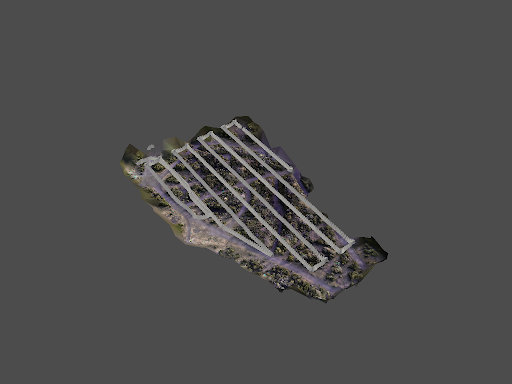
\includegraphics[width=\textwidth]{figs/methods/structure_from_motion/camera estimation.png}
    \caption{The estimated camera locations in space}
    \label{fig:camera-locations}
\end{figure}

These solvers are becoming increasingly robust, and are well-suited to reconstructing scenes captured by drone surveys because the same location is often seen across many images.

\subsection{Online: Simultaneous localization and mapping}
Structure from motion is a powerful tool, but a key limitation is that it can only be used to map the environment after a mission is complete. In settings where a drone is operating autonomously in complex environment such as under the canopy, it is important that it understands where it is in relation to obstacles in real time. This problem is challenging because it requires completing two challenging tasks at once: building a map of the world while estimating where the robot is within the map. This problem is known in the robotics literature as simultaneous localization and mapping (SLAM). This refers to the fact that in a new environment, the robot must build a map of the world at the same time as figuring out where it is in this map. 


Talk about SLOAM \cite{Chen2020SLOAM:Inventory}, a semantic mapping approach specifically for forestry 

%\begin{itemize}
%    \item Should we include more about survey-based methods?
%    
%\end{itemize}


\section{Automated methods for understanding attributes of forests}
Given the increasing amount of raw data about our forests, a key question is how to extract meaningful insights. Quantities such as the extent, species composition, health, or biomass of a forest can be more easily used to make management decisions. Automated processing methods can free domain experts from the laborious task of interpreting this data by hand. There has been a steady shift from methods which are hand-designed to those which use supervised machine learning. This means fitting some sort of model to existing data that shows the input information and the correct interpretation. Then this model can be used to generate predictions on new data. Over the last decade there have been an explosion of approaches relying on deep learning \cite{Lecun2015DeepLearning}, which is a subset of machine learning using models that have multiple hiararchical processing steps. This requires dramatically more parameters than previous machine learning models but allows greater flexability and expressivity. This means that less human intuition is required but also means that large quantities of labeled data are expected to achieve good performance. 



\subsection{Determining Types and Location of Vegitation}
The end goal of an automated forestry system is often to produce a map of where different classes are. Since the predictions are initially made on each image, an important step is inferring the 3D location of these predictions from the 2D image and also resolving disagreeing predictions for the same location. This challenge has been addressed by many approaches in both geospatial and robotics reserach. A key distinction between approaches in these fields is often whether incremental maps need to be produced as the system is running. In geospatial applicaitons, it's often assumed that the data can be processed in a batch after the mission is completed. In robotics context, the content in the environment often informs the exploration, so the maps must be built in realtime. 

Davila et. al. uses a high-precision GPS-INS to register images \cite{Davila2022ADAPT:AI}


\subsection{Understanding What is in Images}
Semantic segmentation is the task of assigning a classification label to every pixel in an image. In the forestry domain, these classes could be broad, such as trees, shrubs, and grasses or more granular, such as different species of trees. An example image can be seen in Figure \ref{fig:background:semantic_seg_example}.

\begin{figure}
    \centering
    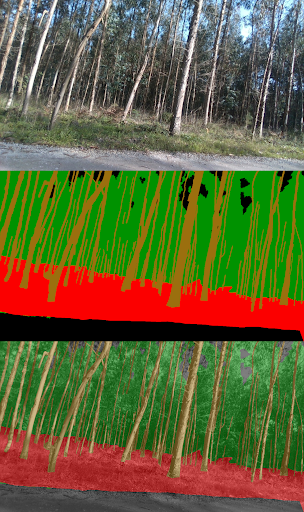
\includegraphics[width=0.45\textwidth, trim={0 340px 0 0}, clip]{figs/background/automated_understanding/segmentation_example.png}
    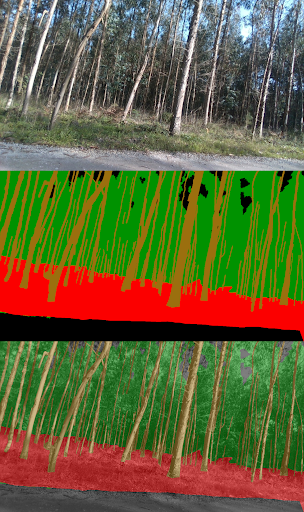
\includegraphics[width=0.45\textwidth, trim={0 170 0 170}, clip]{figs/background/automated_understanding/segmentation_example.png}
    \caption{A visualization of the goal of semantic segmentation. The input image is on the left, and the desired output is on the right, color-coded by class. Red is understory fuel, green is canopy, brown is trunk, and black is background such as bare earth and sky}
    \label{fig:background:semantic_seg_example}
\end{figure}

An early work on semenatic segmetation with deep learning was Fully Convolutional Network \cite{Shelhamer2017FullySegmentation} which took early insights from image classificaiton and adapted them to give per-pixel class predictions. Shortly following this was U-Net \cite{RonnebergerUNET2015}, which had an encoder-decoder architecture with skip connections to preserve high-resolution details. A wide variety of approaches have been developed since then using slight variations on these initial concepts. A recent shift has been toward using transformers \cite{Vaswani2017AttentionNeed} which has resulted in work such as Segformer \cite{Xie2021} and SegNext \cite{Guo2022SegNeXt:Segmentation}.

A signifcation fraction of semantic segmentation works were evaluated on datasets related to autonmous vehicles, sch as CityScapes \cite{Cordts2016}. However, these methods have been shown to be applicable to other domains, and recent work has explored them in the context of drone forestry images \cite{Nogueira2017SemanticConvNets, Neves2020SemanticU}. 


There are a variety of different approaches to semantic mapping that assume different sensors, goals, and domains \cite{Kostavelis2015SemanticSurvey}.
A common toolbox for generic semantic mapping Kimera \cite{Rosinol2020} that provides many different approaches.

To the best of our knowledge, one of the first works that explores semantic mapping in a forestry context is \cite{Andrada2022IntegrationRoboticsb}. This work also studies identifying forest fire fuel   

\begin{itemize}
    \item Talk about what we mean by semantic mapping 
    \item Talk about some generic approaches: UFO map \cite{Duberg2020UFOMap:Unknown}, Kimera 
    \item Our semantic mapping \cite{RussellUnmannedMitigation} that was derived from \cite{semantic_slam_RGBD}
    \item Talk about land-use mapping approaches from ecologists \cite{Liu2018DeepClassification} 
\end{itemize}


\subsection{Detecting Trees from Over-Canopy Data}
A key first step in many ecological modeling applications is understanding the location and extent of individual trees. Because of this, the problem of detecting trees in drone and satellite has recieved signifcant attention. There are a variety of approaches and one way to classify them is whether they use geometric or visual information about the scene. 

Talk about CHM approaches

We chose to use DeepForest \cite{Weinstein2020DeepForest:Delineation} in this work because it's a commonly-used approach that was trained on a diverse set of trees from the national ecological observation network (NEON) \cite{Keller2008ANetwork} across the country.

Talk about DetectTree2 \cite{DetectTree2} \\
Go through Derek's paper and find other ones.

\section{Planning informative drone surveys}

In many forestry applications, the region of interest is commonly substantially larger than what is feasible to survey, either by hand or even with a drone. In practice, foresters  select a small set of plots to visit and extrapolate from these sparse observations to the entire region. These plots are chosen using expert knowledge of the region to be diverse and representative.

Despite the ability of drones to cover much large regions than humans alone, they still fall short of the ability to perform  exhaustive coverage. For example, rough calculations suggest that it would take a drone pilot 250 full days flying to survey the TODO region. Therefore, it is clear that judicious use of limited resources is critical.

Satellite or aerial data is the primary modality of data that scales to the extent required for understanding forests at scale. Unfortunately, prior work has shown that many existing satellite prediction models are highly inaccurate \cite{}. Furthermore, useful global models exist only for select satellite data product and for common tasks like biomass estimation. Therefore, they are not applicable when improved satellites are launched or if a regional satellite or aerial campaign is conducted.
It is possible to tackle fine-grained tasks such as species classification with satellite data, but they are often only relevant to a small region \cite{Sweden}. 
Therefore, we wish to streamline the process of developing satellite prediction models by using a generic framework and fitting it to local observations.

Specifically, we assume that our drone collects data that can be accurately interpreted to predict the quantity of interest. For example, we can task a human annotator with identifying tree species from high-resolution drone images, or train a deep learning model to do the same. We further assume that information relavent to this task is contained in remote sensing data of the scene, but it's not easy or scalable to label this data directly. This may be because a human labeller does not possess the intuition to label species based solely on low-resolution satellite data. This claim is especially relevant if the remote sensing data contains channels other than Red-Green-Blue, as it is hard for humans to fully interpret this data \cite{Hard to label multispectral}.

Given these assumptions, the goal is to choose a set of sample locations to observe with the drone. From these observations, we obtain a classification label for each observed pixel in the remote sensing data. We then train a satellite prediction system using these observed pixels as the ground truth training examples. The goal of this work is to observe regions which serve as useful training samples for this satellite prediction system. This is similar to the ideas of active learning \cite{Ren2022ALearning}, where a repository of unlabeled data is available and an algorithm can query an oracle for labels of a subset of samples. However, active learning is not directly applicable to our domain since in classical formulations, any combination of samples can be selected. In this work, the samples relate to spatial regions that must be visited by a drone. Therefore, it must be possible to visit all the requested samples subject to operational constraints such as the drone's battery life.

This problem is most closely related to prior work in informative path planning (IPP). This diverse field is concerned with how and were to sample observations with an agent to gain some understanding of a phenomena of interest. Due to the diversity of application domains which have their own specific objectives, assumptions, and constraints, there are a diversity of approaches tackling this broad problem. For our domain, a desirable informative path planning algorithm:

\begin{itemize}
    \item \textbf{Considers non-spatial features:} Since we assume that we have prior satellite or low-resolution aerial data of a scene, it is important that an intelligent algorithm leverages this information.
    \item \textbf{Plans over a long horizon:} The commodity drones considered in this work must execute a plan developed prior to launch, e.g. offline, and cannot replan in-flight.
    Therefore, it is important that the algorithm can produce a plan which can be executed for many observations sequentially, ideally as many as can be taken before the battery must be replaced. 
    \item \textbf{Is computationally fast and scalable:} We desire that this algorithm can be executed on a laptop in the field to enable easy deployment.
    To be operationally useful, it must be possible to develop a plan for a new---potentially large---region in a short period of time.
    \item \textbf{Considers area measurements:} Many informative path planning algorithms assume that an observation is a single point in space. Instead, we want to plan were to observe with a downward-facing camera or where to survey a small region. In either case, these observations cover a region that is too large to be approximated as a single point.
\end{itemize}



\subsection{Online methods}

Significant work has been done under the assumption that the agent can re-plan its trajectory online, based on the observations it sees during execution. This requires a sophisticated robotic platform that can sense its environment, process this data into a useful format, re-plan which regions would be useful to explore, and execute this plan. In most cases, the agent maintains some sort of belief of which regions uncertain, desirable, or combination of both. At each re-planning iteration, the agent seeks to develop a plan that is likely to optimize its objectives within the operational constraints such as path length.

The work of \cite{Popovic2020} proposes a generic framework for terrain monitoring with UAVs equipped with a downward facing camera. This work assumes that the quantity of interest is a scalar field defined over the environment that has spatial correlations, e.g. similar locations will have similar values. The example use-case is modeling the density of weeds in an agricultural application, where it is most important to accurately model regions with a high infestation. Further, it assumes that the UAV is able to re-plan its trajectory in flight, after taking uncertain measurements of the environment. A strength of this work is that it models the altitude-dependent effects of a drone camera: at higher altitudes the camera can observe more area but the quality of the measurements will be lower. Using an optimization-based framework and a probabilistic sensor model, the algorithm plans a sequence of observations that decrease the uncertainty while focusing on regions of high predicted weed density. This first part of this path is followed until a new plan based on new observations is developed. This approach is shown to be more effective than a uniform coverage plan at a fixed altitude because it can predict which regions will have more weeds and spend more of the sensing budget there. An extension of this work \cite{Stache2021AdaptiveSegmentation} further explores these concepts with real data. Specifically, they use semantic segmentation to identify weeds in the images and fit empirical models to the segmentation accuracy at different altitudes. This work also shows higher accuracy than a non-adaptive baseline. In both cases, a fundamental strength of the approach is the reason we cannot use it in our domain---online re-planning based on the observed data is critical to the performance increase over the baseline.

A key feature of the previous work is that it seeks to model only regions that were observed with the drone. The main decision is how many times to re-observe a region and at what altitude. In our setting, we wish to make observations with a drone and extrapolate beyond them with satellite data. This goal is somewhat related to that of \cite{Ruckin2022}, which seeks to plan a drone flight that collects images to train a deep learning model for land use classification. In this setting, it is assumed that the drone has a downward facing camera that observes a scene. It also possesses a deep learning model that predicts the land use for each pixel, as well as a measure of uncertainty about the prediction. The goal is to collect images, that when labeled by a human annotator after the mission, can be used to update the model the deep learning model so its performance is better on new data. The authors show that collecting images that the current model is uncertain about leads to better performance after retraining. Therefore, when the drone is collecting data, it should prioritize images that the current model is uncertain about. As the drone explores a region, it generates the uncertainty predictions for each observed images, but cannot access the true label. Then, it continuously updates plan that tries to observe new uncertain images, by assuming that unobserved images next to uncertain observed images will also be uncertain. As with the prior work, this approach requires online reasoning to be effective. Furthermore, this approach has a subtly different goal from ours: their goal is to collect images that can be used to train a good model for new drone observations whereas our approach assumes a model exists already for drone data and these predictions can be used to inform a satellite model. 

Some prior work formulates the problem in similar way to our objective. Work by Kodule et. al. \cite{Kodgule2019Non-myopicMeasurements} and an extension by Candela et. al. \cite{Candela2020PlanetaryMapping} explore the problem of where to gather information with a planetary robot, e.g. Mars Rover, given that the whole region has already been observed by a low-fidelity orbiting satellite. Specifically, it is assumed that the world is represented as a grid of pixels each containing a multispectral (8-channel) observation. Then, multiple Gaussian Processes \cite{Rasmussen2004} are defined which uses the spectral values at each pixel as well as the spatial location of each pixel as features. The goal of 

%Due to the assumption of prior imagery, we may leverage approaches from \cite{Candela2021}, which uses an MCTS planner to explore a world for which prior satellite data exists. This work uses a Gaussian Process to model a quantity of interest. It is challenging to directly apply this work because it assumes that each pixel can be regressed individually by the Gaussian Process. This assumption is unlikely to be correct for high spatial and low spectral resolution data since texture within a local neighborhood will likely need to be considered.

%that can be used to gather information to train a good model for satellite data
%Alberto's Planetary , Alberto's Coral \cite{Candela2021}
%Yogi's Coral \cite{Jamieson2020ActiveEnvironments},


\subsection{Offline/batch methods}
\begin{itemize}
    \item \textbf{Ergodic} Ananya's sparse sensing \cite{Rao}
    \item \textbf{Generic} Sankalp's \cite{Arora2017RandomizedConstraints}, Daniela Rus' Correlated orienteering \cite{Yu2016CorrelatedTasks}
    \item \textbf{TIGRIS} \cite{Moon2022TIGRIS:Planning}
    In this work the authors use a sampling based approach. The chance of taking a sample is biased toward those locations which have higher information content. Importantly, this work takes into account the s
\end{itemize}

Ergodic planning, specifically sparse-sensing ergodic planning \cite{Rao}, provides a framework to plan samples over an \textit{information map} which describes how likely each sample is to be valuable. We could derive this information map from the current model prediction in multiple ways. For example, we could specify that samples predicted as rare classes or extreme AGB values are more interesting. Or we could estimate model uncertainty using ensembles or monte-carlo dropout. However, this approach only considers a per-sample interestingness and spatial diversity of samples. In this case, diversity of appearance may matter more than diversity of location. 



\begin{table}[]
\resizebox{\columnwidth}{!}{%
\begin{tabular}{|l|l|l|l|l|l|}
\hline
 & \makecell{Sparse \\ Ergodic \\ Sensing \cite{Rabbi2020Small-ObjectNetwork}} & \makecell{Optimization-\\based \\ replanning \cite{Popovic2017OnlineUAVs}} & TIGRIS \cite{Moon2022TIGRIS:Planning} & \makecell{MCTS on \\ GPs \cite{Candela2020PlanetaryMapping}} & Proposed \\ \hline
\makecell{Non-spatial \\ features} & X & X & X & Y & Y \\ \hline
\makecell{Long horizon} & Y & X & Y & Y & Y \\ \hline
\makecell{Fast \& scalable} & Y & Y & Y & X & Y \\ \hline
\makecell{Area \\ measurements} & X & Y & Y & Y & Y \\ \hline
%\makecell{Incorporates \\ non-trivial \\ dynamics} & Y & Y & Y & N & N \\ \hline
\end{tabular}%
}
\caption{A comparison of the capabilities of existing informative path planning algorithms.}
\label{tab:my-table}
\end{table}

We can apply concepts from online approaches to offline approaches
We can close the gap between online and offline approaches 

